\section{Assignment 3}
\label{ass3}
\subsection{Implement the Kalman filter/predictor and estimate the velocity and acceleration from noisy position measurements}

Both the Kalman filter and the Kalman predictor are based on the stochastic LTI system:

\begin{equation*}
\begin{cases}
\textbf{x}_{k+1}=A\textbf{x}_k+Bw_k\\
y_k=C\textbf{x}_k+v_k
\end{cases}\;\;\;\;\textbf{x}=\begin{bmatrix}
x\\\dot x\\\ddot x
\end{bmatrix}\;\;\;
A=\begin{bmatrix}
1 & T_s & \frac{T_s^2}{2}\\
0 & 1 & T_s\\
0 & 0 & 1
\end{bmatrix}\;\;\; B=\begin{bmatrix}
\frac{T_s^3}{6}\\\frac{T_2}{2}\\T_s
\end{bmatrix}\;\;\; C=\begin{bmatrix}
1 & 0 & 0
\end{bmatrix}
\end{equation*}

and $w_k$, $v_k$ zero mean uncorrelated Gaussian random variables describing respectively model and noise variances:

\begin{equation*}
w_k=\mathcal N(0,Q)\;\;\;\;v_k=\mathcal N(0,R)
\end{equation*}

with $Q=qBB^T$, $R=var(x)$, $q=10^7$ and initial state $x_0\approx\mathcal N(\bar x_0,P_0)$, $\bar x_0=\begin{bmatrix}
0 & 0 & 0
\end{bmatrix}^T, P_0=\mathbb{I}_3\cdot 1\cdot 10^{-5}$.

The Kalman filter is recursively defined as follows:
\begin{align*}
\hat x_{k+1\mid k+1}&=A\hat x_{k\mid k}+K_{k+1}(y_{k+1}-CA\hat x_{k\mid k})\\
P_{k+1\mid k}&=AP_{k\mid k-1}A^T-AP_{k\mid k-1}C^T(CP_{k\mid k-1}C^T+R)^{-1}CP_{k\mid k-1}A^T+Q
\end{align*}

where $P$ is the variance of the estimation error and the Kalman gain (the matrix that maps the output estimation error into the correction of the state) defined as:
\begin{equation*}
K_{k+1}=P_{k+1\mid k}C^T(CP_{k+1\mid k}C^T+R)^{-1}
\end{equation*}

The Kalman predictor is recursively defined as follows:
\begin{align*}
\hat x_{k+1\mid k}&=A\hat x_{k\mid k-1}+\bar K_{k}(y_{k}-C\hat x_{k\mid k-1})\\
P_{k+1\mid k}&=AP_{k\mid k-1}A^T-AP_{k\mid k-1}C^T(CP_{k\mid k-1}C^T+R)^{-1}CP_{k\mid k-1}A^T+Q
\end{align*}

with the Kalman gain defined as:
\begin{equation*}
\bar K_{k}=AP_{k\mid k-1}C^T(CP_{k\mid k-1}C^T+R)^{-1}
\end{equation*}

The difference between filter and predictor is that the former estimates the state $\hat x$ at time $k+1$ given measurements until time $k+1$, while the latter estimates the state $\hat x$ at time $k+1$ given measurements until time $k$ (1-step ahead prediction). Therefore the resulting estimations will differ only in the first state. Both filter and predictor are applied to a position signal with Gaussian noise and a signal with quantization noise. The results are shown in figures \ref{fig:kalman_fp_gauss} and \ref{fig:kalman_fp_quant}.

\subsection{Implement the steady-state Kalman filter/predictor and estimate the velocity and acceleration from noisy position measurements}

The steady state Kalman filter and predictor are obtained by computing a fixed solution for the estimation error variance $P_{\infty}$ and for the Kalman gain, $K_{\infty}$. The estimation error variance for $k\to\infty$ is obtained by solving the Algebraic Riccati Equation:

\begin{equation*}
P_\infty = AP_\infty A^T-AP_\infty C^T(CP_\infty C^T + R)^{-1}CP_\infty A^T + Q
\end{equation*}

Then, the Kalman gains for the filter and predictor are defined as:

\begin{equation*}
K_\infty = P_\infty C^T(CP_\infty C^T+R)^{-1}\;\;\;\;\bar K_\infty = AP_\infty C^T(CP_\infty C^T+R)^{-1}
\end{equation*}

Finally, the steady state Kalman filter is defined as:

\begin{equation*}
\hat x_{k+1\mid k+1}=A\hat x_{k\mid k}+K_\infty(y_{k+1}-CA\hat x_{k\mid k})
\end{equation*}

while the steady state Kalman predictor is defined as:

\begin{equation*}
\hat x_{k+1\mid k}=A\hat x_{k\mid k-1}+\bar K_\infty(y_{k}-C\hat x_{k\mid k-1})
\end{equation*}

Both filter and predictor are applied to a position signal with Gaussian noise and a signal with quantization noise. The results are shown in figures \ref{fig:kalman_fp_gauss} and \ref{fig:kalman_fp_quant}.

\begin{figure}[H]
\centering
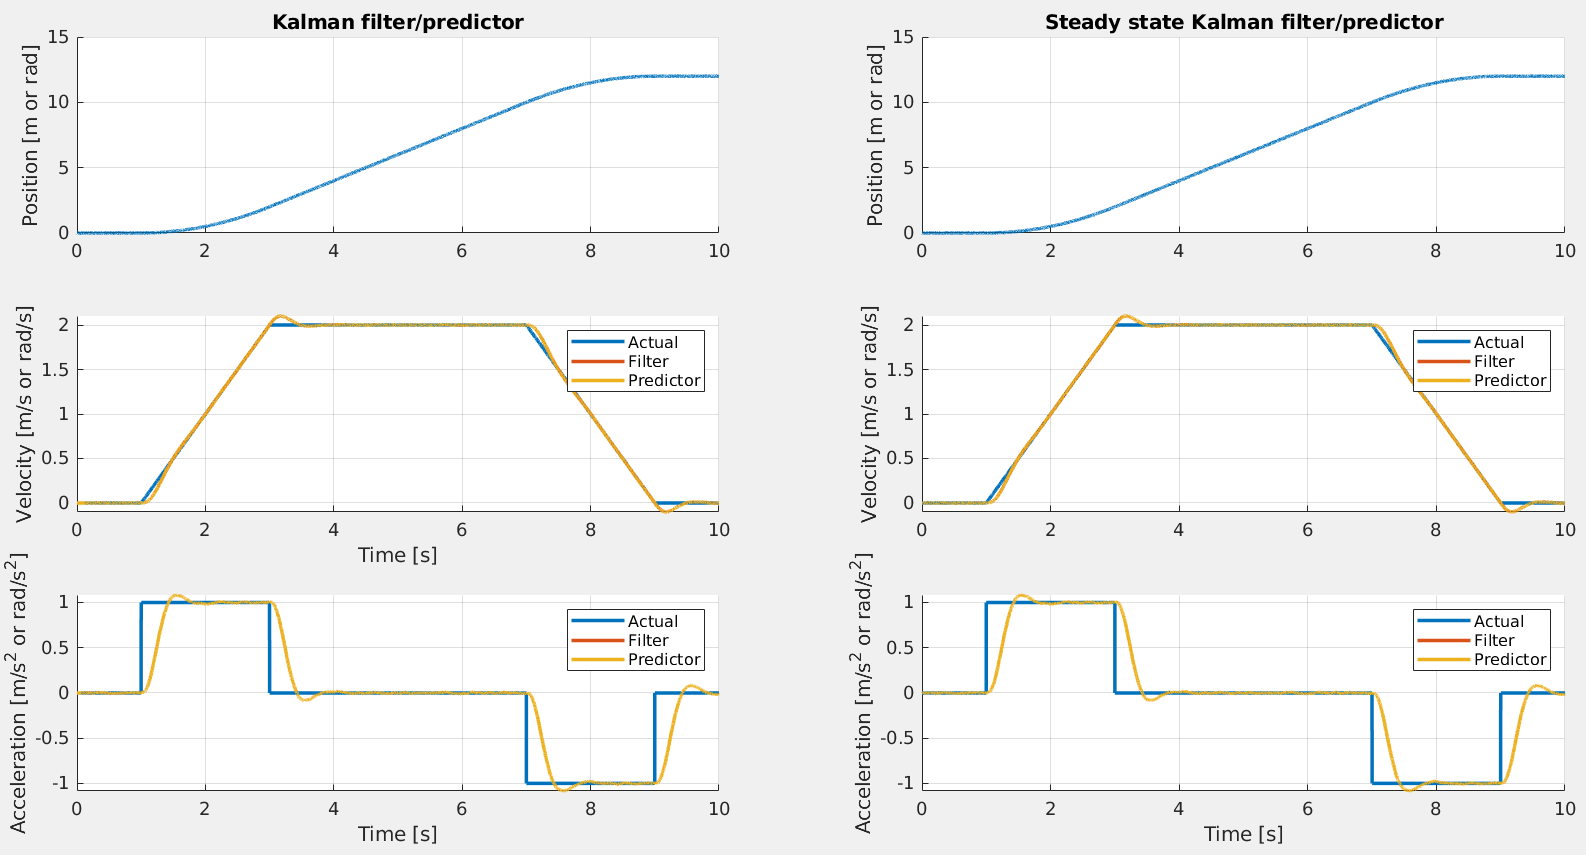
\includegraphics[keepaspectratio,width=\textwidth]{kalman_fp_gauss}
\caption{Kalman filter/predictor applied to a position signal with Gaussian noise}
\label{fig:kalman_fp_gauss}
\end{figure}

\begin{figure}[H]
\centering
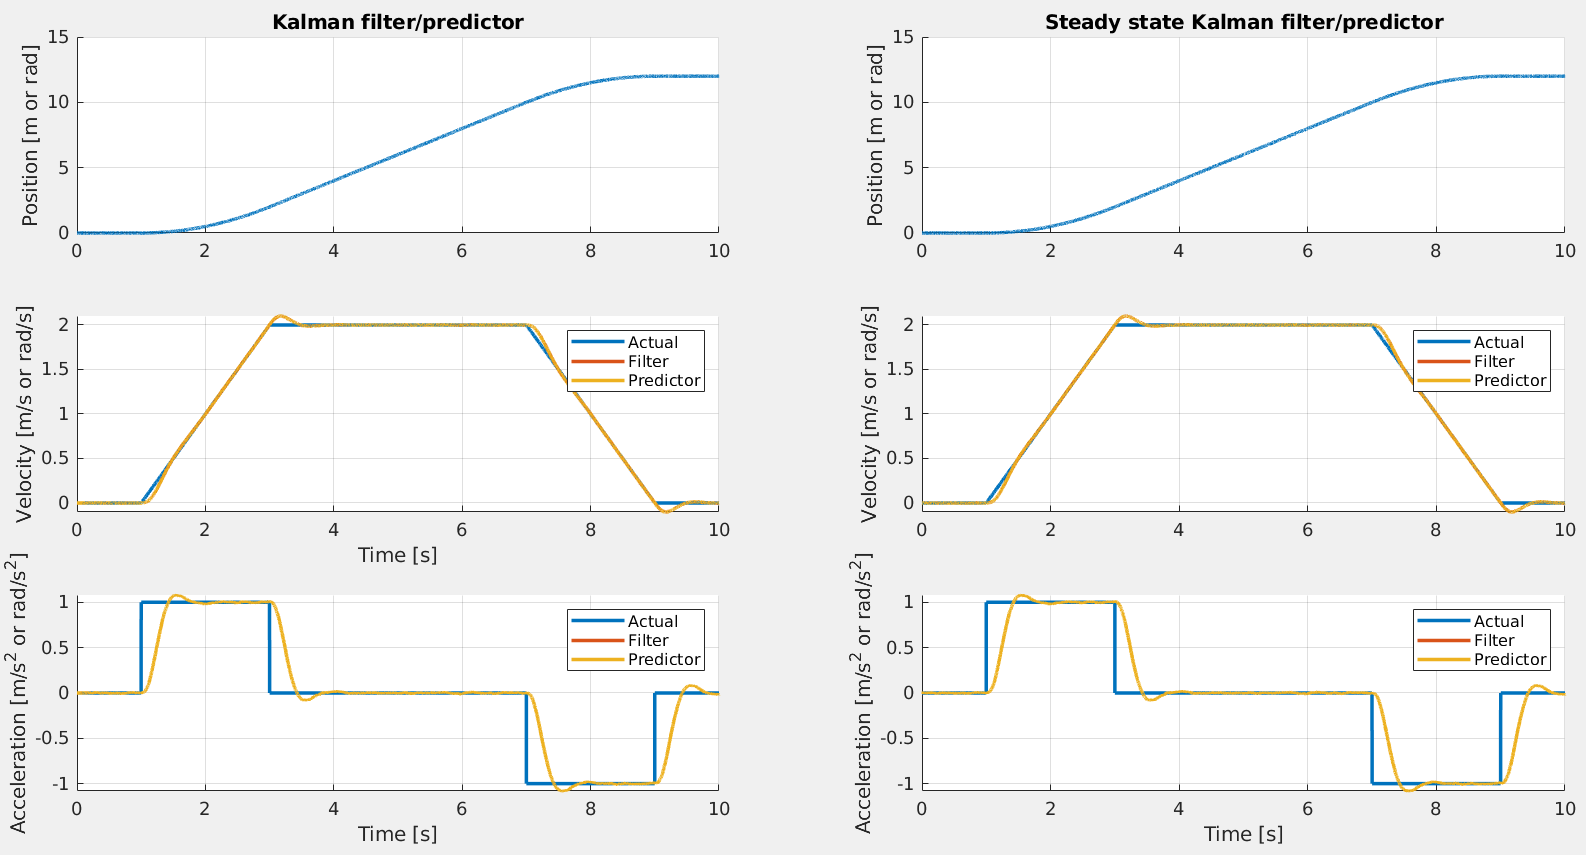
\includegraphics[keepaspectratio,width=\textwidth]{kalman_fp_quant}
\caption{Kalman filter/predictor applied to a position signal with quantization noise}
\label{fig:kalman_fp_quant}
\end{figure}

As expected, both filter and predictor produce the same estimations, and there's no difference with their respective steady-state implementations. Both the Gaussian and quantization noise cases produce very similar estimates.